\subsection{Кластеризация}
Данные были кластеризованы алгоритмами иерархической и спектральной кластеризации с параметрами, определёнными в главе 2. Ниже показана дендрограмма, полученная в результате кластеризации.
\begin{figure}[H]
	\center
  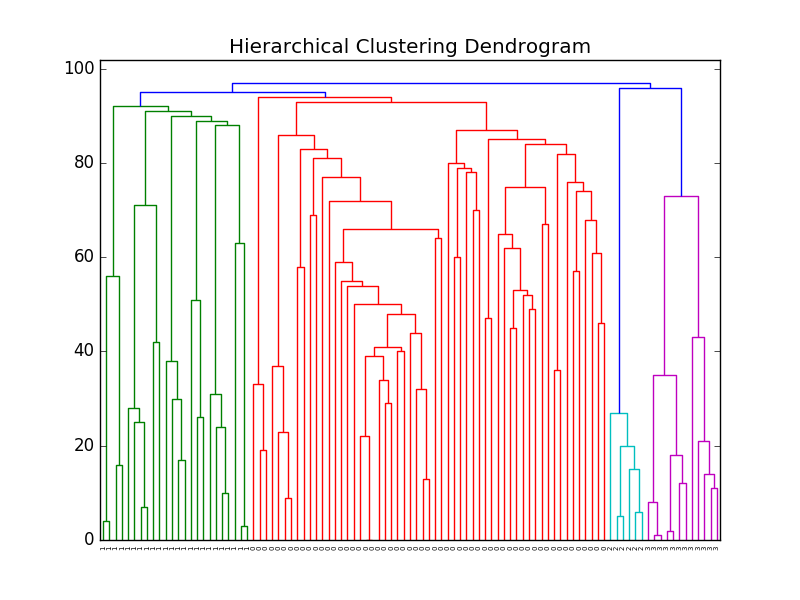
\includegraphics[width=0.75\linewidth]{pics/original_normalized.png}
  \caption{Дендрограмма кластеризуемых данных}
  \label{dendrogram_experimental}
\end{figure}

Следуя критерию большего интервала, иерархическая кластеризация формирует четыре кластера, что показано на дендрограмме \ref{dendrogram_experimental}. Визуализируя результаты спектральной кластеризации с помощью t-SNE на рисунке \ref{tsne_experimental} можно подтвердить этот вывод.
\begin{figure}[H]
	\center
  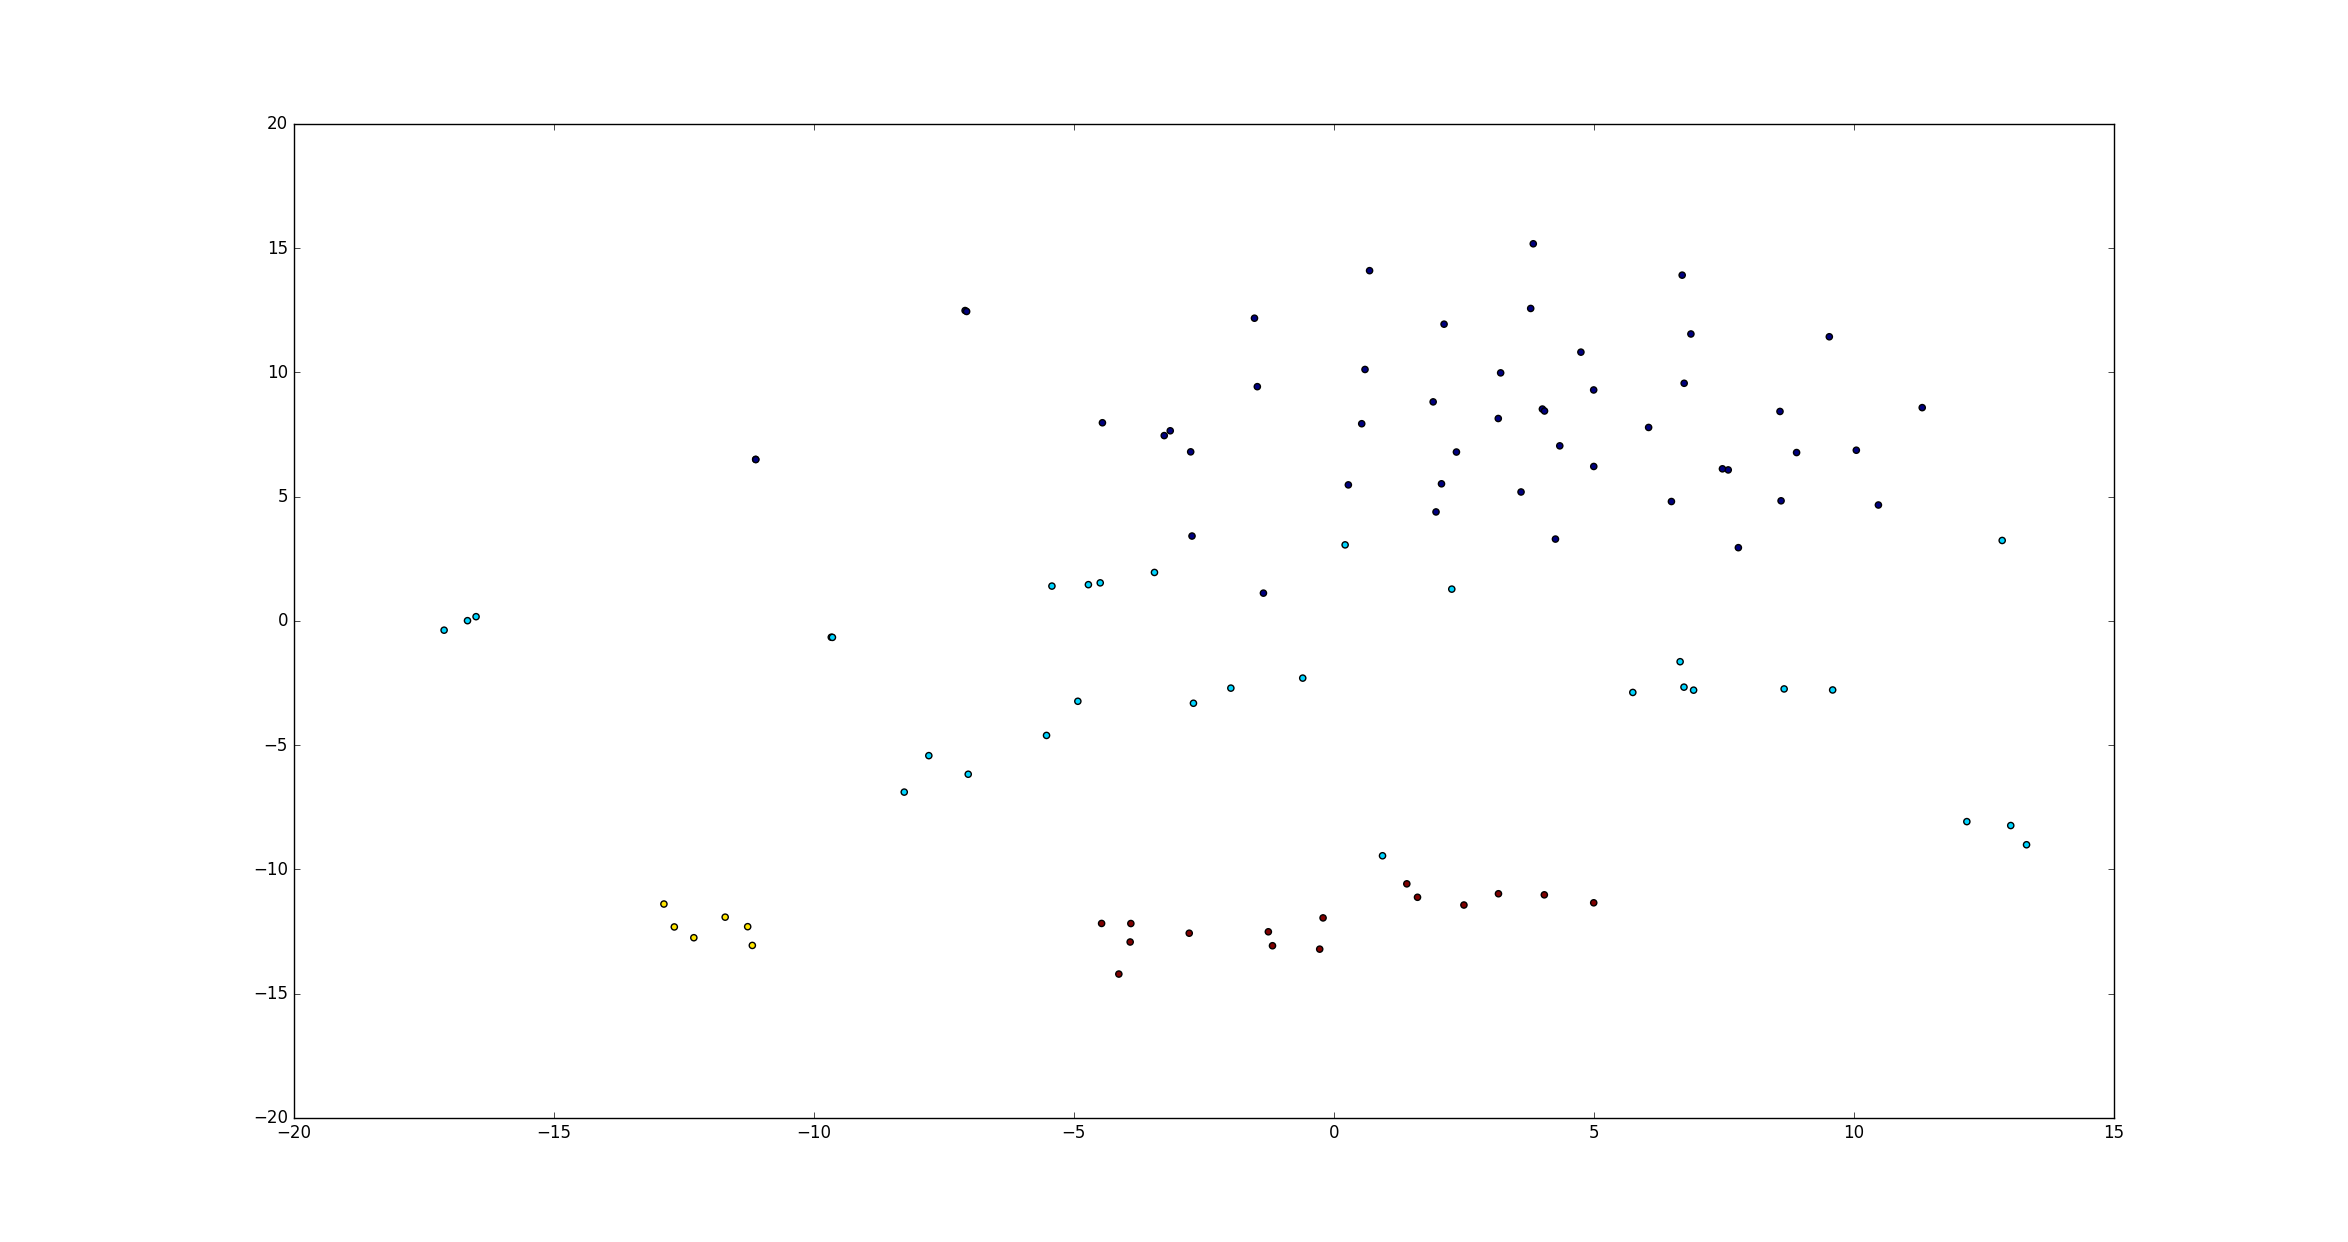
\includegraphics[width=\linewidth]{pics/tsne_color_experimental.png}
  \caption{Визуализация экспериментальных данных с помощью t-SNE}
  \label{tsne_experimental}
\end{figure}

Данное разбиение далее используется в качестве эталонного.

\subsection{Отбор признаков генетическим алгоритмом}
Генетический алгоритм, чьи параметры были определены в главе 2, был запущен на экспериментальных данных. Результатом отбора стали 35 признаков, кластеризация на которых полностью повторяет эталонную. Количество признаков, отобранное генетическим алгоритмом выбрано в качестве базового уровня для оценки ражирующих алгоритмов. 

Перечень отобранных признаков: highECI\_Motif\_1, CCC, ACGT, ACTC, AGAA, AGAC, AGAG, AGCA, AGCC, AGCG, AGCT, AGGA, AGGG, AGTG, ATCA, CACC, GGAG, TGTA, AAAAC, AAGAC, ACCGC, ACGGA, AGCTC, ATCGG, CACCA, CACTC, CCCGT, CTCAG, CTGAA, CTTGT, GCGCC, GGTCT, TACAC, TAGGC, TATAG

\subsection{Ранжирование признаков с применением спектральной теории графов}

\subsubsection{Оригинальный показатель важности}

\begin{figure}[H]
	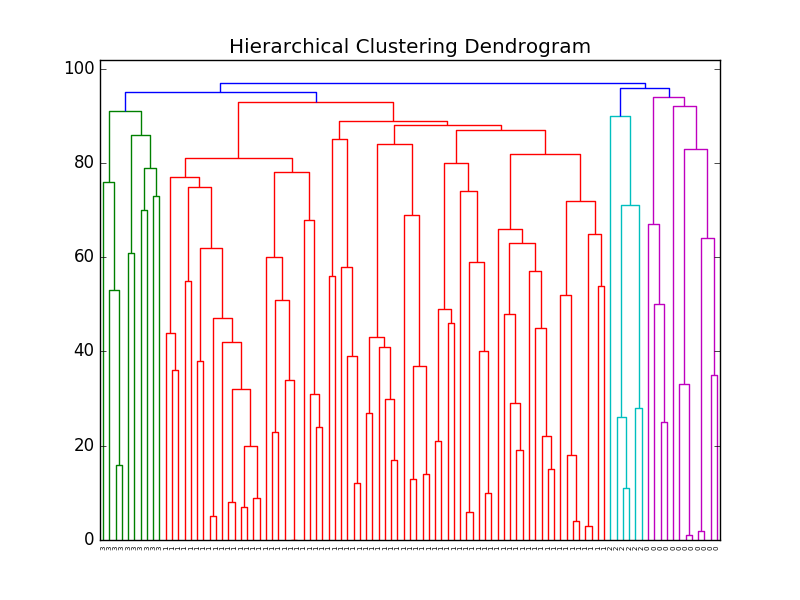
\includegraphics[width=0.5\linewidth]{pics/dendrograms/lp_norm_cosine.png}
	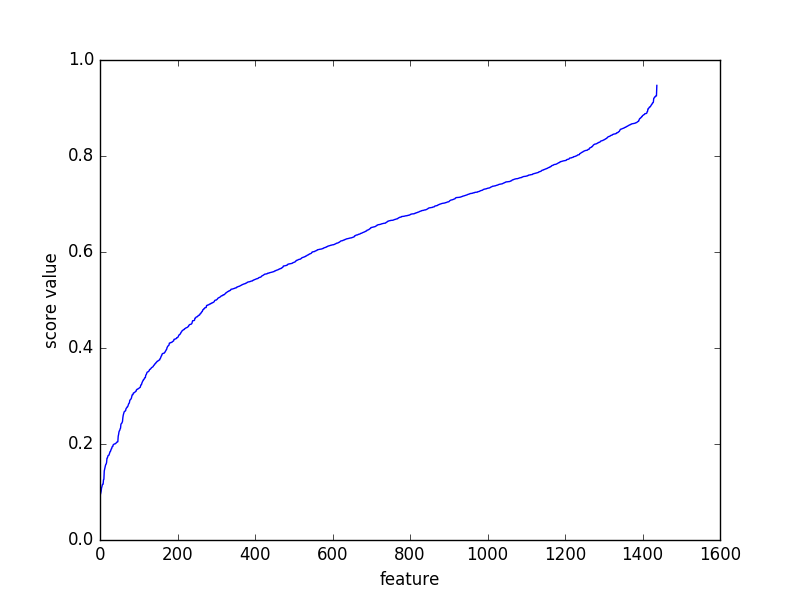
\includegraphics[width=0.5\linewidth]{pics/graphs/lp_norm_cosine.png}
	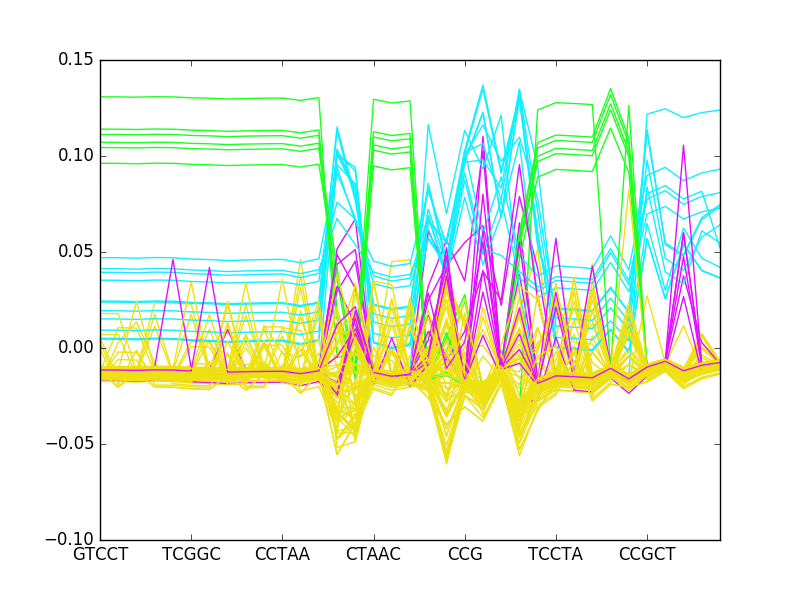
\includegraphics[width=0.5\linewidth]{pics/profiles/lp_norm_cosine.png}
	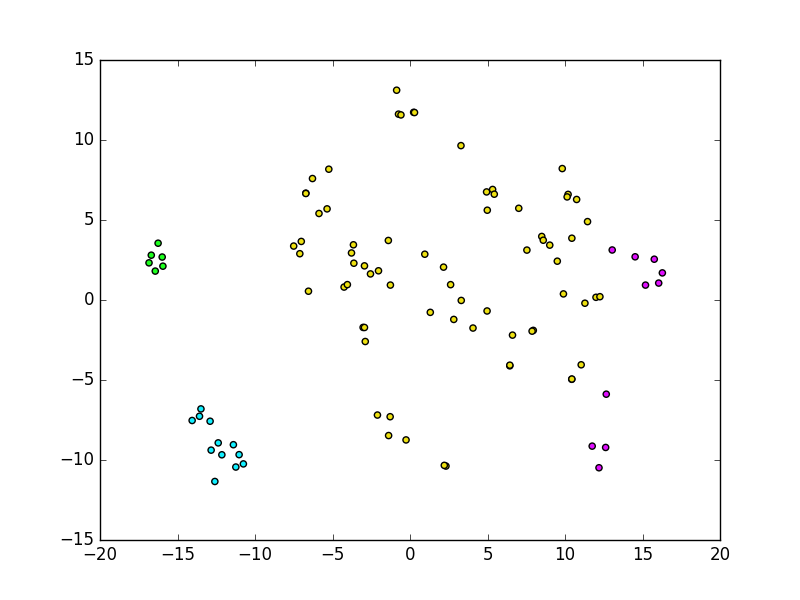
\includegraphics[width=0.5\linewidth]{pics/tsne/lp_norm_cosine.png}
	\caption{График важности признаков, дендрограмма кластеризации, t-SNE визуализация и профили экзонов на 35 наиболее важных признаках при оригинальном показателе важности на предобработанных данных}
	\label{lp_norm_cosine}
\end{figure}


\begin{figure}[H]
	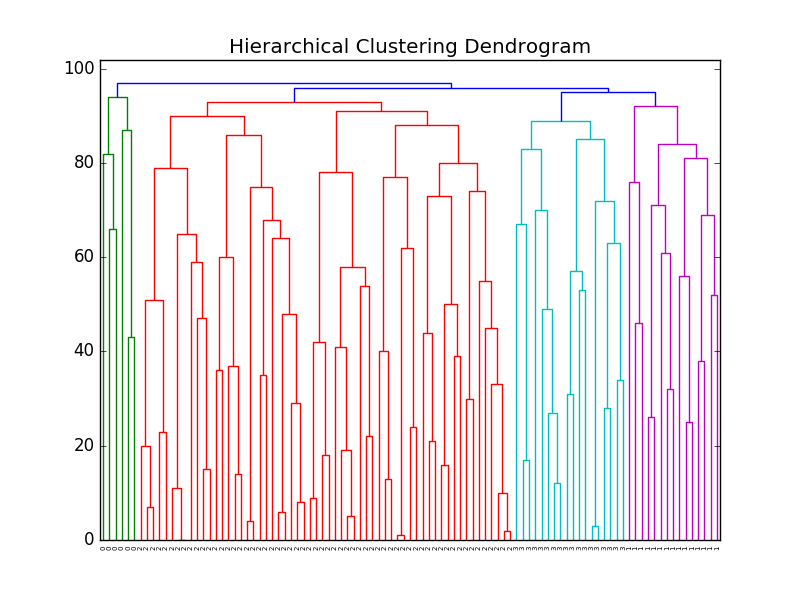
\includegraphics[width=0.5\linewidth]{pics/dendrograms/lp_unnorm_cosine.png}
	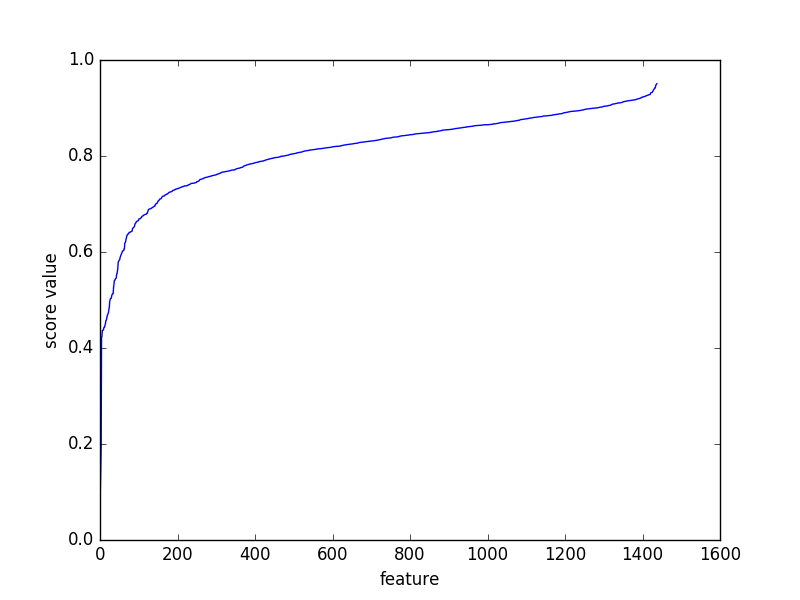
\includegraphics[width=0.5\linewidth]{pics/graphs/lp_unnorm_cosine.png}
	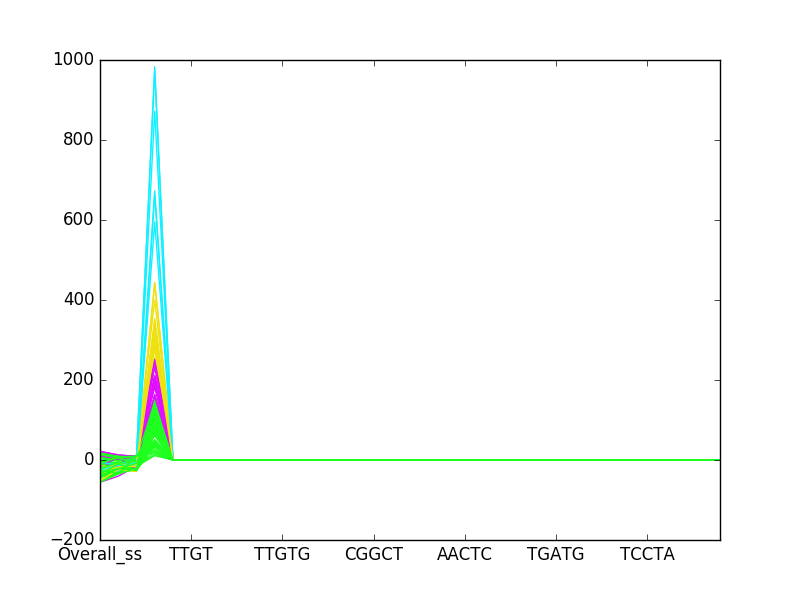
\includegraphics[width=0.5\linewidth]{pics/profiles/lp_unnorm_cosine.png}
	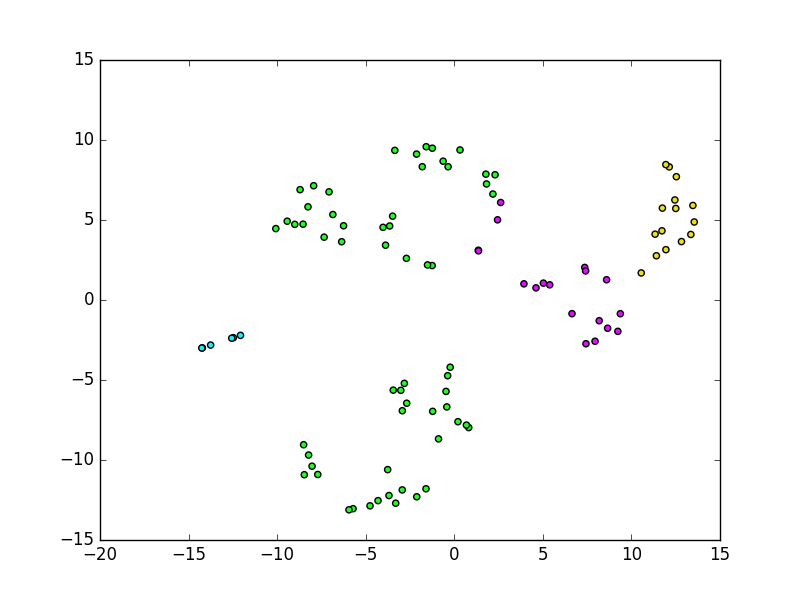
\includegraphics[width=0.5\linewidth]{pics/tsne/lp_unnorm_cosine.png}
	\caption{График важности признаков и дендрограмма кластеризации, t-SNE визуализация и профили экзонов на 35 наиболее важных признаках при оригинальном показателе важности на оригинальных данных}
	\label{lp_unnorm_cosine}
\end{figure}

\subsubsection{Использование ядер}

\begin{figure}[H]
	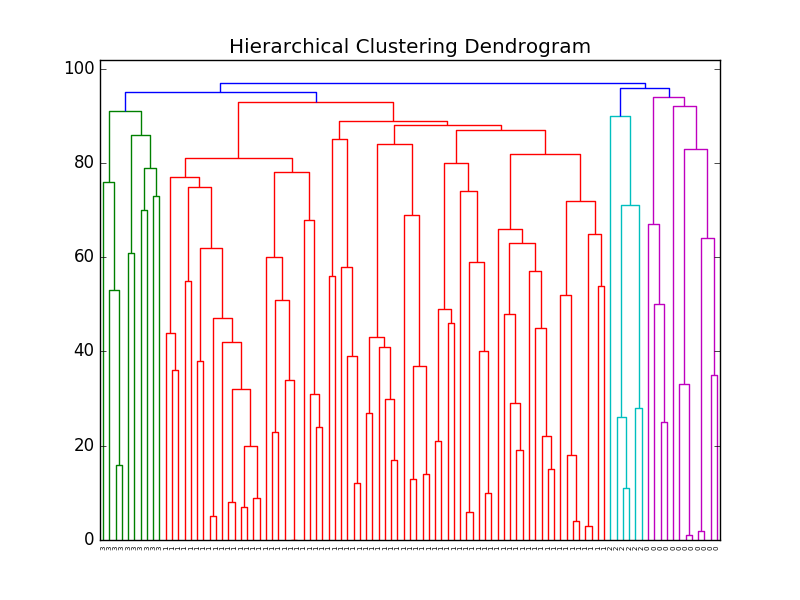
\includegraphics[width=0.5\linewidth]{pics/dendrograms/spec_norm_cosine.png}
	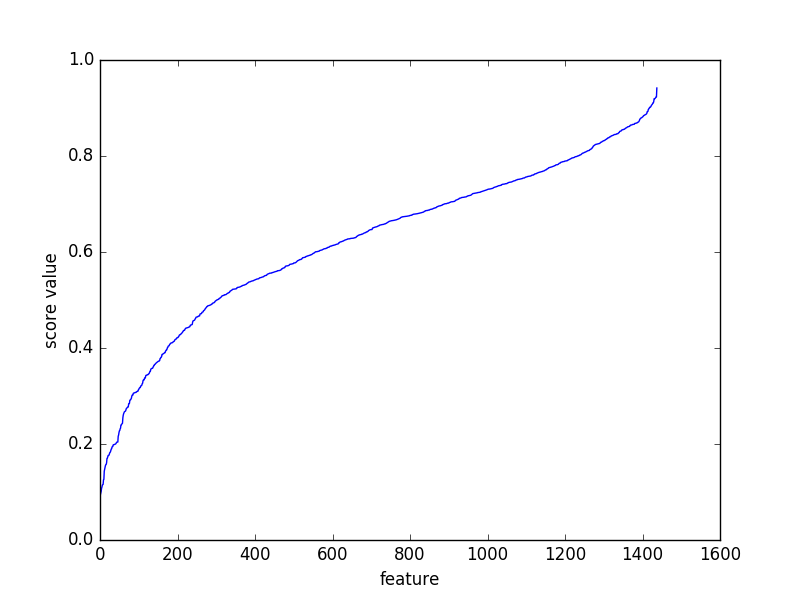
\includegraphics[width=0.5\linewidth]{pics/graphs/spec_norm_cosine.png}
	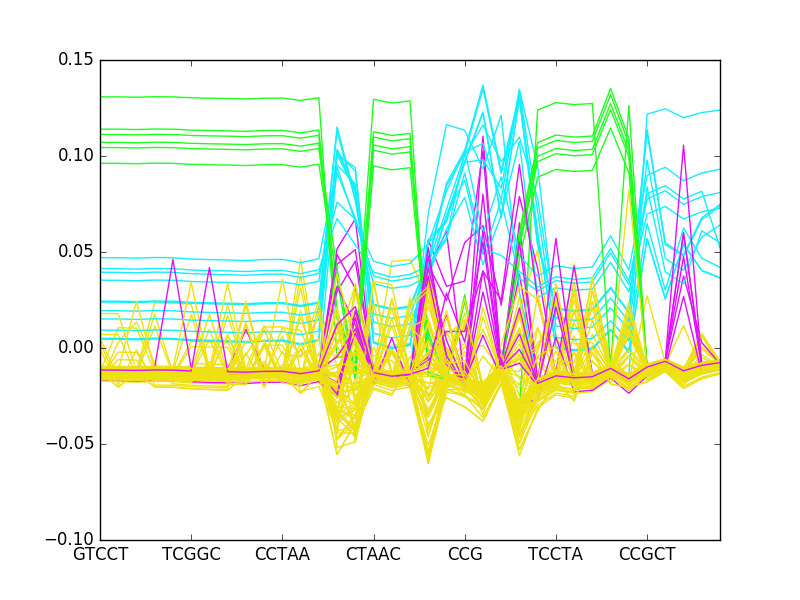
\includegraphics[width=0.5\linewidth]{pics/profiles/spec_norm_cosine.png}
	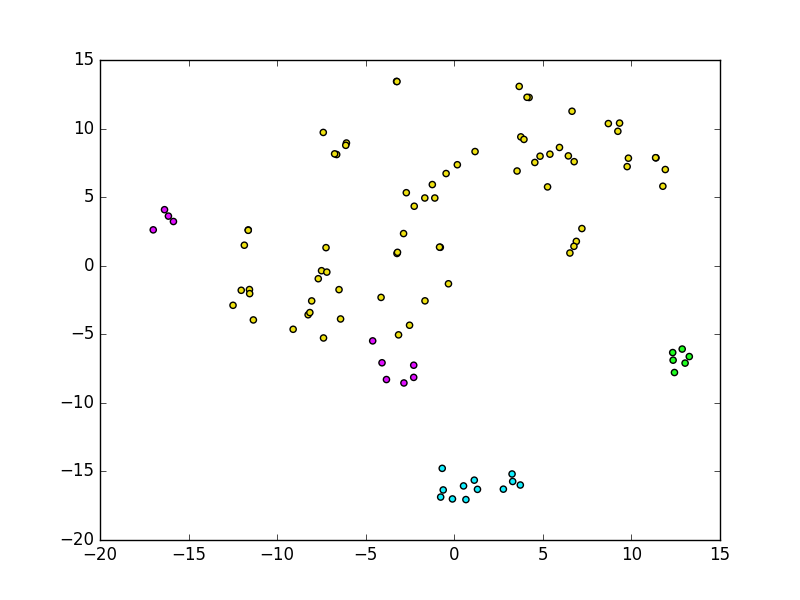
\includegraphics[width=0.5\linewidth]{pics/tsne/spec_norm_cosine.png}
	\caption{График важности признаков, дендрограмма кластеризации, t-SNE визуализация и профили экзонов на 35 наиболее важных признаках при показателе важности c ядром на предобработанных данных}
	\label{spec_norm_cosine}
\end{figure}


\begin{figure}[H]
	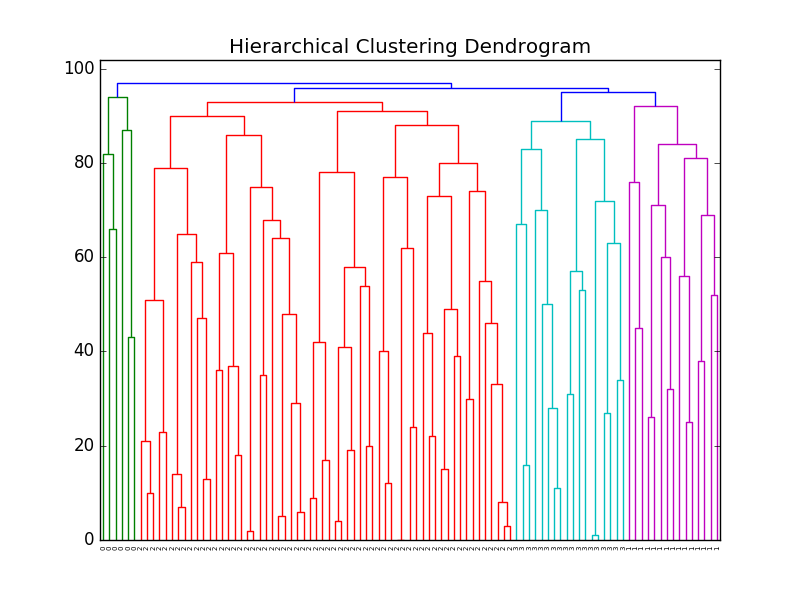
\includegraphics[width=0.5\linewidth]{pics/dendrograms/spec_unnorm_cosine.png}
	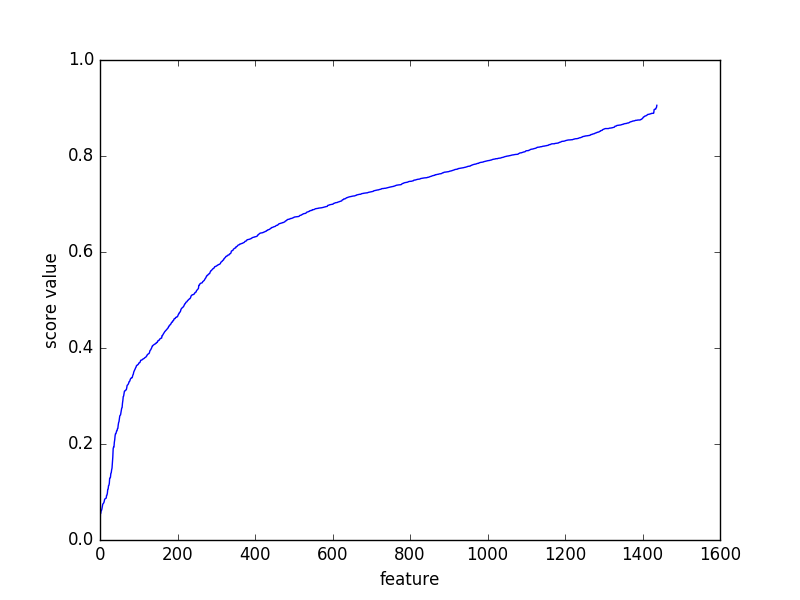
\includegraphics[width=0.5\linewidth]{pics/graphs/spec_unnorm_cosine.png}
	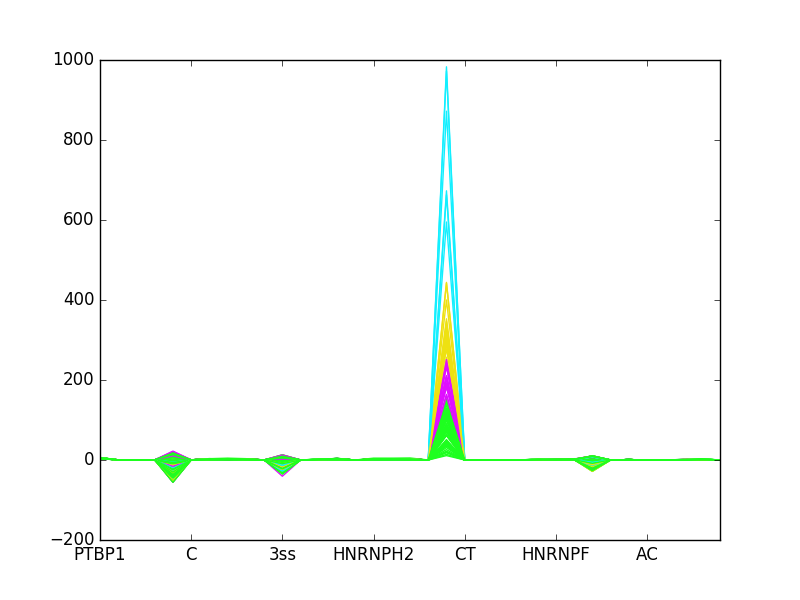
\includegraphics[width=0.5\linewidth]{pics/profiles/spec_unnorm_cosine.png}
	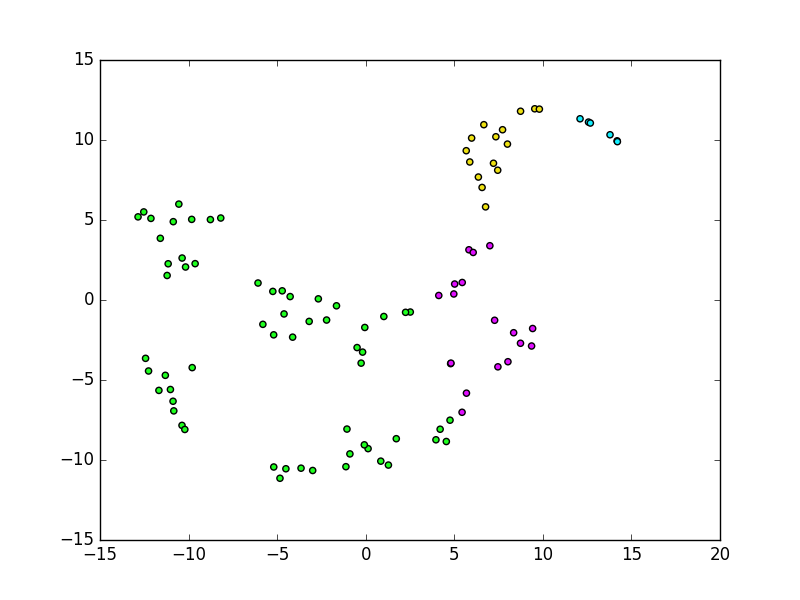
\includegraphics[width=0.5\linewidth]{pics/tsne/spec_unnorm_cosine.png}
	\caption{График важности признаков, дендрограмма кластеризации, t-SNE визуализация и профили экзонов на 35 наиболее важных признаках при показателе важности с ядром на оригинальных данных}
	\label{spec_unnorm_cosine}
\end{figure}

\subsubsection{Использование регуляризации и покластерного отбора признаков}


\begin{figure}[H]
	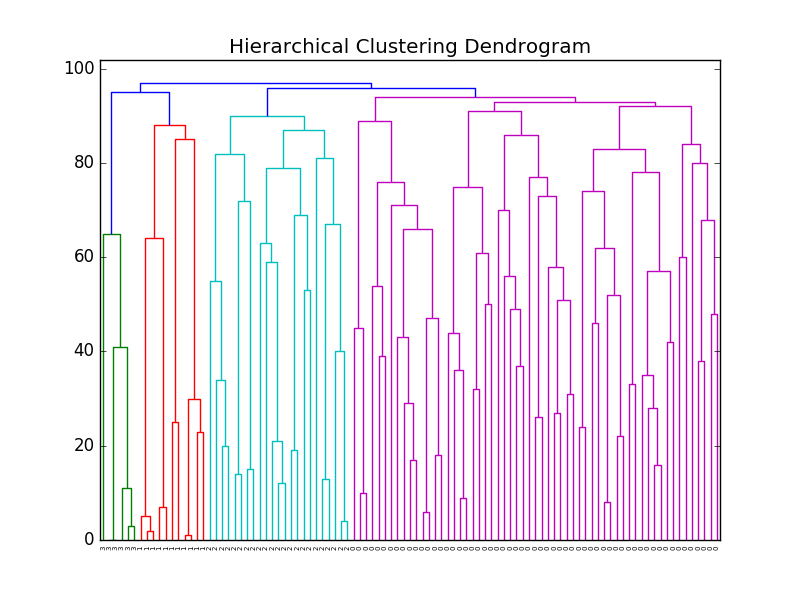
\includegraphics[width=0.5\linewidth]{pics/dendrograms/ndfs_norm_cosine_1c.png} 
	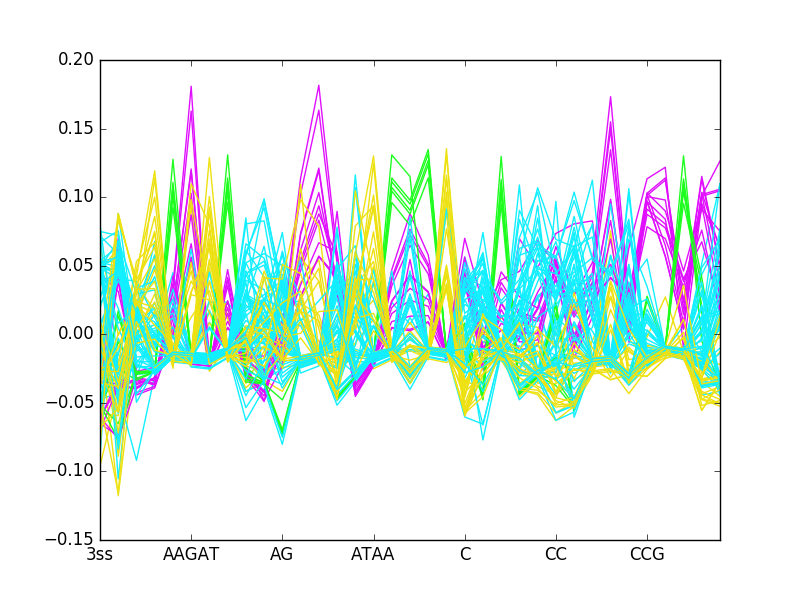
\includegraphics[width=0.5\linewidth]{pics/profiles/ndfs_norm_cosine_1c.png}
	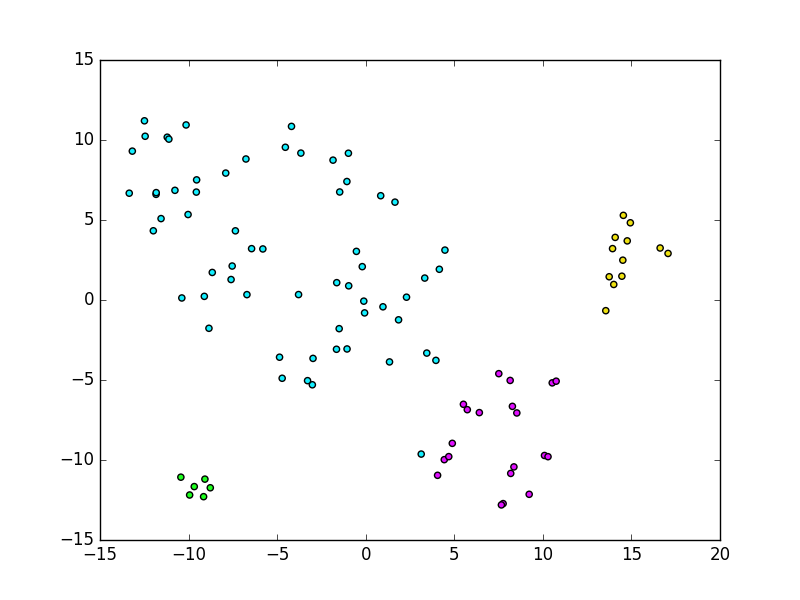
\includegraphics[width=0.5\linewidth]{pics/tsne/ndfs_norm_cosine_1c.png} \\
	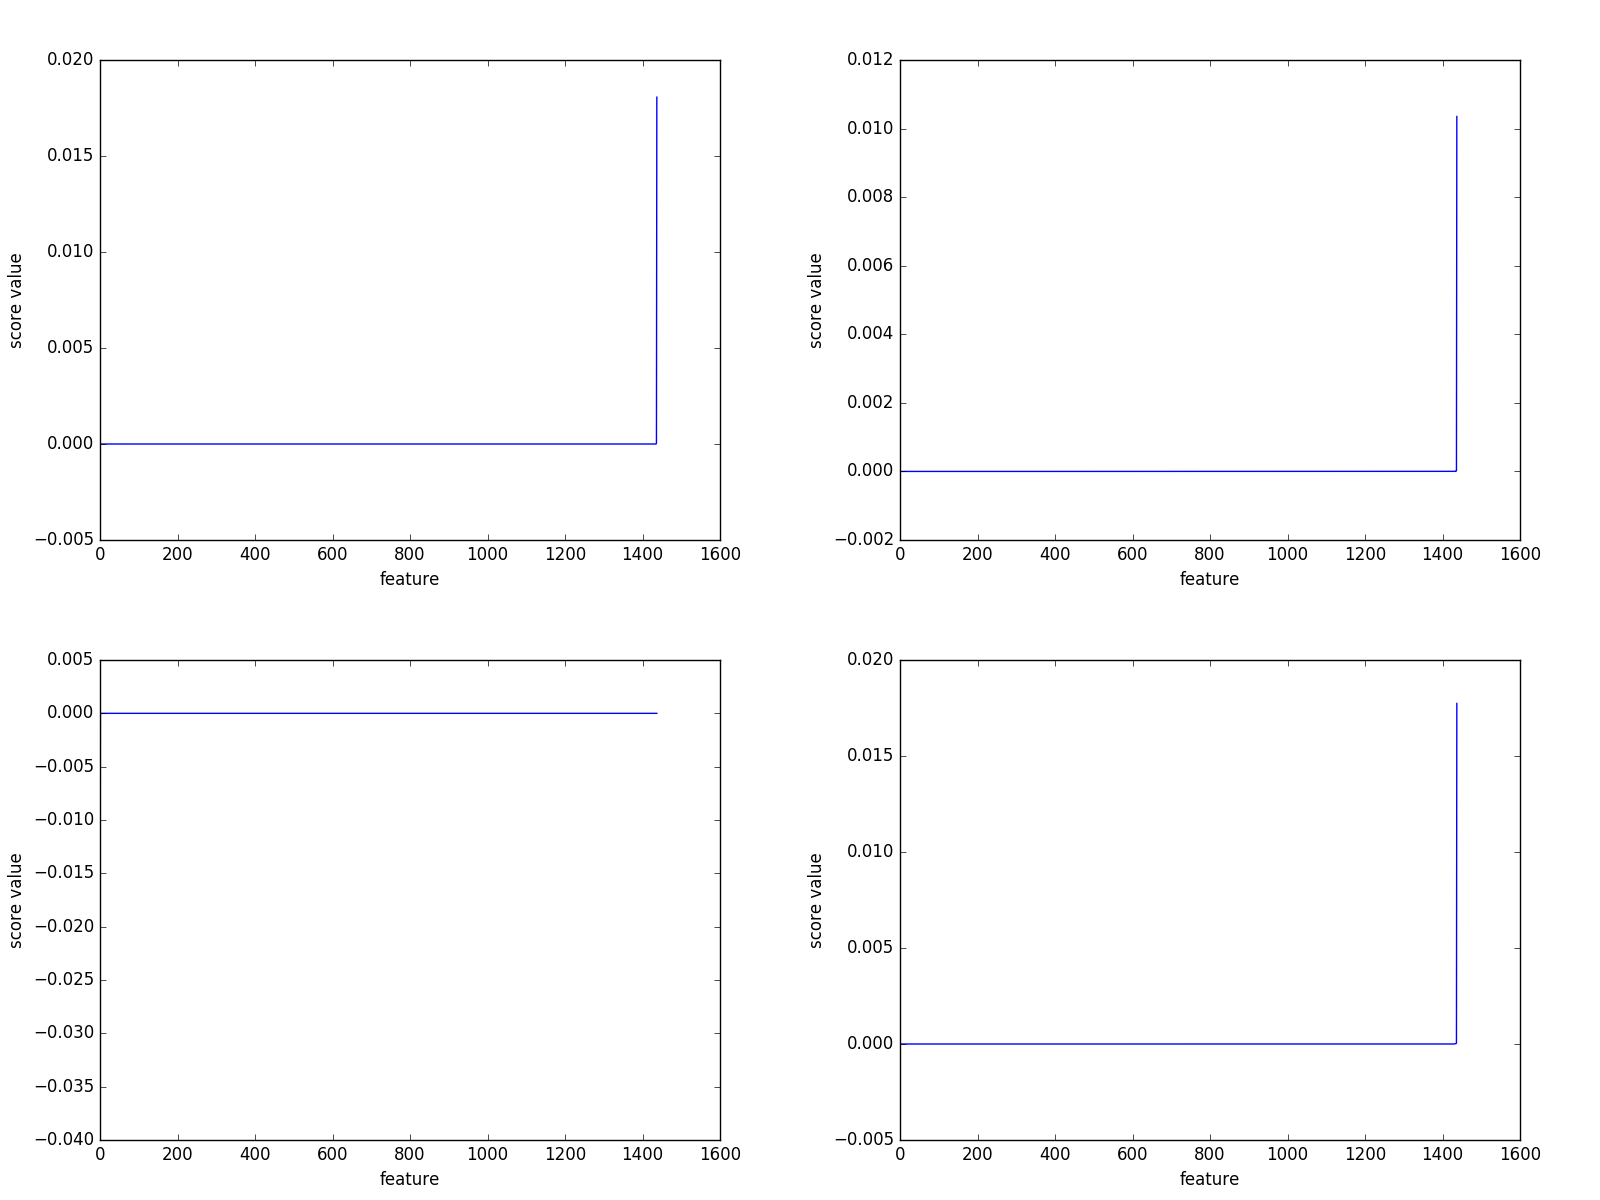
\includegraphics[width=0.8\linewidth]{pics/graphs/ndfs_norm_cosine.png}
	\caption{Покластерный график важности признаков, дендрограмма кластеризации, t-SNE визуализация и профили экзонов на 35 наиболее важных признаках при регуляризованном показателе важности на предобработанных данных}
	\label{ndfs_norm_cosine}
\end{figure}


\begin{figure}[H]
	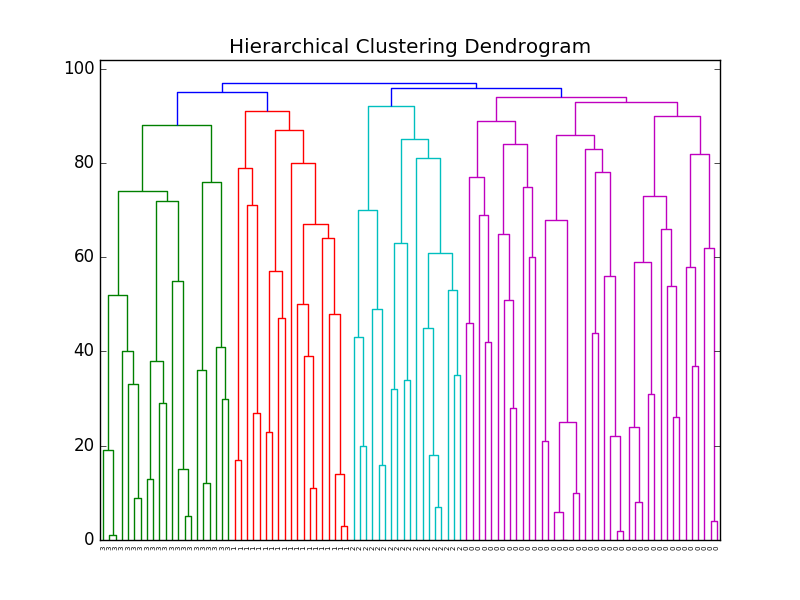
\includegraphics[width=0.5\linewidth]{pics/dendrograms/ndfs_unnorm_cosine_1c.png} 
	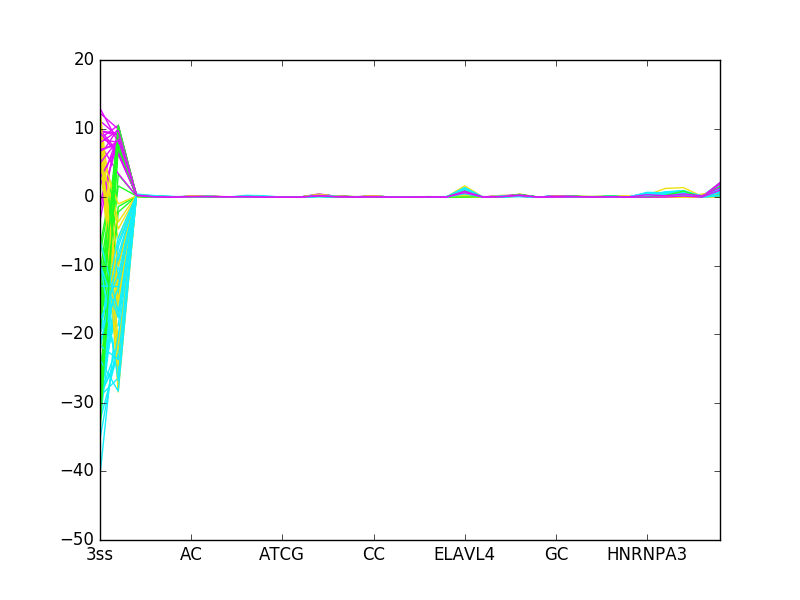
\includegraphics[width=0.5\linewidth]{pics/profiles/ndfs_unnorm_cosine_1c.png}
	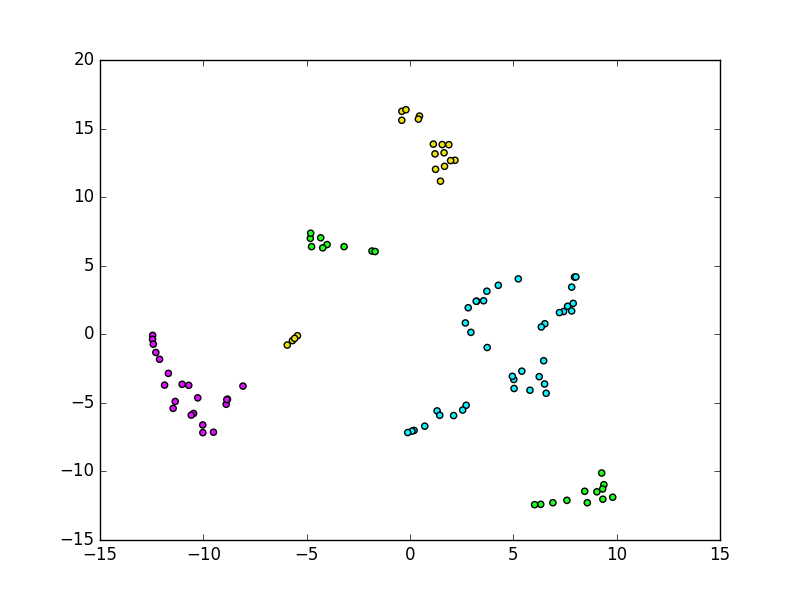
\includegraphics[width=0.5\linewidth]{pics/tsne/ndfs_unnorm_cosine_1c.png} \\
	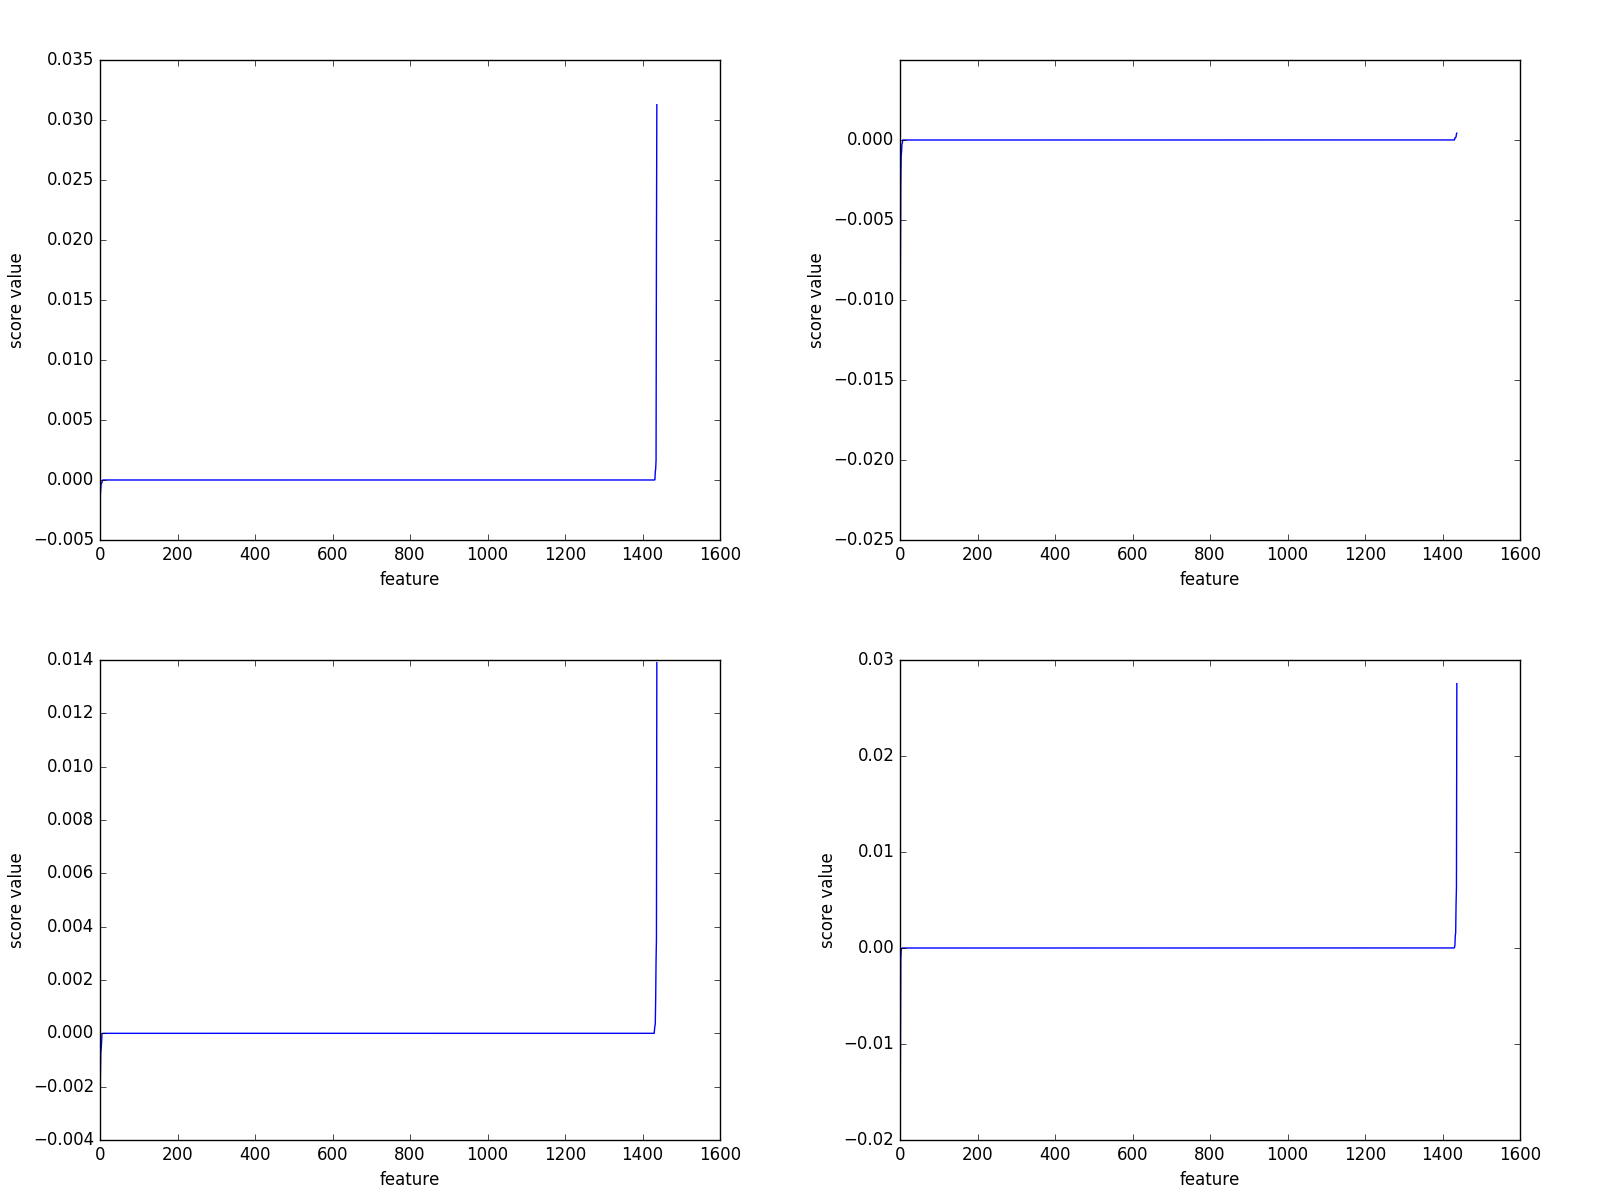
\includegraphics[width=0.8\linewidth]{pics/graphs/ndfs_unnorm_cosine.png}
	\caption{Покластерный график важности признаков, дендрограмма кластеризации, t-SNE визуализация и профили экзонов на 35 наиболее важных признаках при регуляризованном показателе важности на оригинальных данных}
	\label{ndfs_unnorm_cosine}
\end{figure}

\subsubsection{Сравнение отобранных признаков для предобработанных данных}

\begin{longtable}{|c|c|c|c|}
	\hline
	Оригинальный показатель & С ядром & Покластерный & Регуляризованный \\ \hline
	GTCCT & GTCCT & AAT & 3ss \\ \hline
GGGTC & GGGTC & AATGC & AAA \\ \hline
GGTCC & GGTCC & ACGAG & AACTC  \\ \hline
AATCG & AATCG & ACTAC & AAGAT  \\ \hline
ATCGG & ATCGG & ACTCC & AATA  \\ \hline
TCGGC & TCGGC & AGAT & AATCG  \\ \hline
GCTTG & GCTTG & AGATG & AC  \\ \hline
CAATC & CGGCT & AGGC & ACA  \\ \hline
CGGCT & CAATC & AGGCA & ACC  \\ \hline
TTGTG & TTGTG & AGTGG & ACCGC  \\ \hline
CCTAA & CCTAA & ATGTT & AGAT  \\ \hline
TGATG & TGATG & ATTCT & AGATG  \\ \hline
GTTGT & GTTGT & C & AGC  \\ \hline
CG & CG & CAATG & AGT  \\ \hline
GC & GC & CACCT & ATAA  \\ \hline
CTAAC & CTAAC & CACGA & ATCGG  \\ \hline
AACTC & AACTC & CAGAC & ATGC  \\ \hline
CTCAA & CTCAA & CGAG & ATGCG  \\ \hline
CGC & C & CGC & ATGTT  \\ \hline
C & CGC & CGGCT & ATT  \\ \hline
CCG & CCG & CTCA & C  \\ \hline
GCGC & GCGC & CTCC & CA  \\ \hline
GCCG & GCCG & CTCCA & CAATC  \\ \hline
GCG & GCG & CTTA & CAC  \\ \hline
CGGC & CGGC & GACTA & CACC  \\ \hline
TCCTA & TCCTA & GATGC & CC  \\ \hline
GGGT & TCGG & GC & CCA  \\ \hline
TCGG & GGGT & GGCAA & CCACC  \\ \hline
GCGTA & GCGTA & GGTCC & CCAGG  \\ \hline
TGTGA & TGTGA & GTAGA & CCG \\ \hline
CCGCT & CCGCT & GTCCT & CCGCT  \\ \hline
CCGCG & CCGCG & GTTGT & CCTAA  \\ \hline
CGAGC & CGAGC & MFE & CG  \\ \hline
CCGC & CCGC & SRSF9 & CGA  \\ \hline
GCCGC & GCCGC & TA & CGAG  \\ \hline
\caption{35 наиболее важных признаков для каждого подхода на предобработанных данных}
\label{features_norm}
\end{longtable}

\subsubsection{Сравнение отобранных признаков для оригинальных данных}

\begin{longtable}{|c|c|c|c|}
	\hline
	Оригинальный показатель & С ядром & Покластерный & Регуляризованный \\ \hline
Overall\_ss & PTBP1 & 3ss & 3ss \\ \hline
3ss & G & AACA & 5ss \\ \hline
5ss & T & AAGCT & A \\ \hline
Length & A & ACCGG & AA \\ \hline
AATCG & Overall\_ss & ACTC & AAA \\ \hline
TTGT & C & AGAG & AAAA \\ \hline
CCTAA & YBX1 & AGCTT & AAC \\ \hline
GTCCT & HNRNPH1 & AGG & AG \\ \hline
GTTGT & HNRNPK & AGGCA & AGG \\ \hline
GGGTC & TG & AGGG & AT \\ \hline
TTGTG & 3ss & AGGGG & ATCG \\ \hline
GGTCC & CA & ATCTT & ATGC \\ \hline
CTTGT & SFPQ & CAATG & C \\ \hline
CTCAA & PCBP1 & CAATT & CC \\ \hline
TCGGC & MFE & CCAT & CGTA \\ \hline
CGGCT & HNRNPH2 & CCCTG & CTG \\ \hline
ATCGG & HNRNPH3 & CCGGA & CTGT \\ \hline
TGTTG & MBNL1 & CCTTC & CTT \\ \hline
GCTTG & AG & CGAAA & DAZAP1 \\ \hline
CAATC & Length & CGAGT & ELAVL4 \\ \hline
AACTC & CT & CGCCT & FMR1 \\ \hline
TGT & ESEseqs & CGCGC & Fairbrother \\ \hline
TTGTT & ESSseqs & CGTC & G \\ \hline
TGTT & GA & CGTGG & GA \\ \hline
CTAAC & KHSRP & CTA & GATGC \\ \hline
TGATG & HNRNPF & CTCC & GC \\ \hline
GTGAT & PCBP2 & CTTGT & GCT \\ \hline
GATGC & 5ss & CTTTT & GCTG \\ \hline
CA & TC & GAAAG & GCTT \\ \hline
GGGT & phastCons & GACGG & GG \\ \hline
TCCTA & AC & GAG & GGC \\ \hline
TCAAT & GT & GATGC & GGT \\ \hline
GCGTA & SRSF7 & GCACA & GT \\ \hline
ATGCG & TIA1 & GCTCT & GTG \\ \hline
CGTAT & GG & GGAA & GTGG \\ \hline

\caption{35 наиболее важных признаков для каждого подхода на оригинальных данных}
\label{features_unnorm}
\end{longtable}

\subsection{Оценка отбора признаков алгоритмами из спектральной теории графов}

~

\begin{table}[H]
	\begin{tabular}{|c|c|c|}
	\hline
	Особенность алгоритма & Стандартизированные & Оригинальные \\ \hline
	Изначальный расчет показателя & 0.63 & 0.81 \\ \hline
	Применение степенного ядра & 0.66 & 0.96 \\ \hline
	Регуляризация & 0.85 & 0.07 \\ \hline
	Кластерный тбор признаков &  0.71 & 0.17 \\ \hline
	\end{tabular}
\caption{Взаимная информация для разработанного алгоритма на стандартизированных и оригинальных}
\end{table}

~

Алгоритмы отбора признаков на основе спеткральной теории графов, разработанные в главе 2, были применены к экспериментальным данным. Результаты отбора признаков представлены в таблице. Показано сохранение взаимной информации между эталонной кластеризацией и кластеризацией на 35 наиболее важных признаках. 


\newpage
\section{Основные результаты и выводы}
\begin{itemize}
	\item В главе описано применение разработанного алгоритма к экспериментальным данным
	\item Получены результаты, позволяющие сделать вывод о применимости выбранного подхода к экспериентальным данным
	\item Генетический алгоритм задает хороший базовый уровень для исследуемых алгоритмов, задав 35 признаков, полностью сохраняющих эталонное разбиение
	\item Алгоритмы на основе спектральной теории графов позволяют ранжировать признаки по важности, задавая для каждого значение показателя важности
	\item Исследовано влияние подходов различных алгоритмов к ранжированию признаков
	\item Исследуя влияние применения ядра к лапласиану графа, на рисунках \ref{spec_norm_cosine} и \ref{spec_unnorm_cosine},по сравнению с \ref{lp_unnorm_cosine} и \ref{lp_norm_cosine}, применение ядра не влияет на ранжирование при нормированных данных, но имеет влияние при оригинальных
	\item Регуляризация и внутрикластерный обтбор признаков уменьшают показатель неважных признаков, упрощая интерпретацию результата, что видно сравнивая рисунки \ref{ndfs_unnorm_cosine} и \ref{ndfs_norm_cosine} с \ref{lp_unnorm_cosine} и \ref{lp_norm_cosine}
	\item Для каждого подхода отобраны 35 наиболее важных признаков, что позволяет сравнить результаты работы алгоритмов с отобранными генетическим алгоритмом. Анализ таблиц \ref{features_norm} и \ref{features_unnorm} показывает, что в случае оригинальных данных большое влияние показывают признаки с высокой дисперсией, что подтверждает гипотезу, высказанную в начале главы. Множества признаков, отобранные на предобработанных данных схожи между собой и множеством признаков, отобранным генетическим алгоритмом, что позволяет выделить эти признаки как наиболее важные. 
\end{itemize}